\section{Experiments}
\subsection{Setup}
\subsubsection{Dataset.} 
We evaluate our method on the nuScenes dataset, which contains 1,000 examples of 360° street-view scenes captured by six cameras. Following the official configuration, we utilize 700 scenes (28,130 frames) for training and 150 scenes (6,019 frames) for validation. 
For objects, we focus on ten categories: car, bus, truck, trailer, motorcycle, bicycle, construction vehicle, pedestrian, barrier, and traffic cone. Each category is represented by distinctly colored bounding boxes, which serve as inputs for the box adapter. 
Regarding maps, we concentrate on three primary types: driving area, lane, and pedestrian crossing. These layouts are also color-coded and processed by the map adapter.
\subsubsection{Evaluation Metrics.} 
Following prior works, we evaluate the proposed method based on metrics that measure  generation fidelity and controllable accuracy of objects and roads. 
Specifically, Frechet Inception Distance (FID) is adopted to measure the realism of synthesized images.
For controllability, we test the generated validation set with pre-trained perception models, CVT~\cite{zhou2022cross} and BEVFusion~\cite{liu2022bevfusion}. 
Metrics such as nuScenes Detection Score (NDS), mean Average Precision (mAP), and mean Average Orientation Error (mAOE) are used to quantify alignment with ground truth annotations.
\subsubsection{Implementation Details.}
Our framework builds upon Stable Diffusion 2.1, initializing the UNet with pre-trained weights. 
Training consists of two stages: geometric conditions are learned separately for 60k steps, followed by dual condition adaptation for 10k steps. 
Trade-off weights are set as $\lambda_\text{freq} = 0.5$ for frequency-guided structure loss and $\lambda_\text{MI} = 0.05$ for mutual information constraint.
We use the AdamW optimizer~\cite{loshchilov2017decoupled} with a learning rate of $6 \times 10^{-5}$. During inference, the DDIM sampler~\cite{songdenoising} is configured with 25 steps, and the classifier-free guidance (CFG) scale is set to 3. The resolution of the generated images is $224 \times 480$ pixels.
For multi-view scene descriptions, we leverage Qwen2.5-VL-72B~\cite{bai2025qwen2}, achieving state-of-the-art performance in visual understanding and textual generation. Additional implementation details are provided in the supplementary material.


\begin{table}[t]
	\centering
	\caption{
		Comparison of generation fidelity and controllability across different driving-view generation methods on the NuScenes {validation} set. Panacea* denotes our reproduced results based on the officially provided generated dataset.  Outcomes demonstrating superior performance are highlighted in \textbf{bold}. $\uparrow$ / $\downarrow$ indicates that a higher/lower value is better. }
	% surpasses all baselines throughout the evaluation. 
	\label{table:1}
	\resizebox{\linewidth}{!}{
		\begin{tabular}{@{}lcc|ccc|cc@{}}
			\toprule
			\multirow{2}{*}{Method} & \multirow{2}{*}{\begin{tabular}[c]{@{}c@{}}Synthesis\\ resolution\end{tabular}} & \multirow{2}{*}{FID$\downarrow$} & \multirow{2}{*}{mAP$\uparrow$} & \multirow{2}{*}{NDS$\uparrow$} & \multirow{2}{*}{mAOE$\downarrow$} & Road & Vehicle\\
			&&&&&&mIoU$\uparrow$&mIoU$\uparrow$\\
			\midrule
			Oracle & -- & -- & 35.54 & 41.20 & 0.56 & 73.68 & 34.80  \\
			\midrule
			BEVGen  & --  & 25.54 & -- & -- & -- & 50.20 & 5.89 \\
			BEVControl & 224 $\times$ 400 & 24.85 & -- & -- & -- &  60.80 & 26.80 \\
			MagicDrive & 224 $\times$ 480 & 16.20 & 12.30 & 23.32 & -- &  61.05 & 27.01 \\
			Panacea* & 256 $\times$ 512 & 16.96  & 11.65 & 22.40 & 0.82 & 57.11 & 22.77\\
			PerLDiff & 256 $\times$ 704 & 13.36  & {15.24} & {24.05} & {0.78} & {61.26} & {27.13}\\
			\rowcolor{gray!25} Ours & 224 $\times$ 480 & \textbf{11.45}  & \textbf{15.37} & \textbf{25.49} & \textbf{0.76} & \textbf{63.95} & \textbf{27.82}\\
			\bottomrule
		\end{tabular}
		
	}
\end{table}
\subsection{Main Results}
\subsubsection{Realism Evaluation.}
In the realm of image synthesis, lower FID scores indicate better reconstruction quality of real driving scene styles. As shown in Tab. \ref{table:1}, our method achieves an FID score of 11.45, representing the highest realism among all tested approaches.
Our approach significantly outperforms existing solutions, including MagicDrive and Panacea, and even surpasses the recent state-of-the-art method Perldiff by approximately 16.7\%. This substantial improvement demonstrates that fine-grained hierarchical descriptions are highly effective for scene reconstruction.
\subsubsection{Geometrical Controllability.}
Our method shows remarkable performance in segmentation tasks, achieving a road mIoU of 63.95 and surpassing the second-best method by 2.69 points, as shown in the last two columns of Table~\ref{table:1}. This can be attributed to our progressive learning strategy, which prioritizes learning road layouts prior to objects. Additionally, there is a modest improvement in vehicle segmentation.
In terms of 3D object detection, our approach outperforms previous methods by attaining the highest mAP and NDS scores, indicating strong geometric alignment with ground truth annotations. The reductions in orientation and positioning errors can be attributed to the combined benefits of our frequency-guided structure loss and progressive learning strategy.
\subsubsection{Training Support for BEV Segmentation.}
Generative models have been widely recognized as powerful tools for data augmentation, significantly enhancing the generalization capabilities of perception models. 
To evaluate this potential, we leverage synthesized datasets to improve segmentation performance on the NuScenes test set. 
Since the test dataset lacks annotations for objects except roads, we focus our evaluation on improving road segmentation performance.
The results presented in the second row of Tab.~\ref {Tab.augmentation-35k} demonstrate that augmenting training data with optimally annotated real data (i.e., combining the NuScenes training set with the real validation set) yields substantial performance improvements. 
Furthermore, our synthetic validation set achieves competitive augmentation results that closely approximate the performance gains obtained with real validation data, while significantly outperforming other driving scene generation approaches.
\begin{table}[H]
	\centering
	\caption{
		Performance comparison for the boosting performance of BEV segmentation models using synthesized dataset on the NuScenes \textit{test} set using CVT. 
		The “\textit{train} + Real \textit{val}” configuration serves as a benchmark, representing the ideal upper performance limit achievable. 
		The numbers in parentheses indicate the performance disparity relative to the “\textit{train} + Real \textit{val}” configuration.
	}
	\label{Tab.augmentation-35k}
	\resizebox{0.65\linewidth}{!}{
		\begin{tabular}{@{}l|c@{}}
			\toprule
			Training & Road mIoU$\uparrow$ \\
			\midrule
			\textit{train} & 65.83 \\
			\textit{train} + Real \textit{val} & 67.53 \\
			\textit{train} + Syn. \textit{val} (MagicDrive) & 66.12 {(-1.41)} \\
			\textit{train} + Syn. \textit{val} (Panacea) & 66.60 {(-0.93)} \\
			\textit{train} + Syn. \textit{val} (PerLDiff) & 65.74 {(-1.79)} \\
			\rowcolor{gray!25}\textit{train} + Syn. \textit{val} (Ours) & 67.49 {(-0.04)} \\
			\bottomrule
		\end{tabular}
	}
\end{table}
\subsection{Ablation Study}
\subsubsection{Effectiveness of Component Designs.}
To validate the contribution of each component, we conduct comprehensive ablation studies, as shown in Tab.~\ref{table:ablation}.
We evaluate three key components: Multi-View Hierarchical Descriptions (MHD), Frequency-Guided Structure Loss (FGSL), and Mutual Information Constraint (MIC).
Without any of these components, the vanilla model demonstrates poor generation quality.
In particular, its performance in geometric control is noticeably inferior to prior methods such as MagicDrive.
This indicates that the observed performance improvements stem from the proposed components rather than the T2I-Adapter-based architecture.
Introducing MHD alone significantly reduces the FID to 12.03, while improving Road mIoU to 61.22 and Vehicle mIoU to 26.49. This indicates that richer textual inputs provide more detailed semantic guidance, thereby enhancing both image realism and scene controllability.
Applying FGSL independently also yields substantial improvements, with FID reduced to 14.47, Road mIoU increased to 62.92, and Vehicle mIoU reaching 26.95. The gains in controllability metrics, particularly over MHD alone, indicate that the emphasis on high-frequency details effectively refines the structural generation of roads and objects.
Combining MHD and FGSL leads to further performance gains, reducing FID to 11.68 while improving both segmentation metrics. 
Finally, incorporating MIC helps the model better adapt to the joint conditioning of HD maps and 3D bounding boxes, achieving the best overall performance.
\begin{table}[t]
	\centering
	\caption{
		Ablation study on the effectiveness of Multi-View Hierarchical Descriptions (MHD), Frequency-Guided Structure Loss (FGSL), and Mutual Information Constraint (MIC) in driving scene generation.
	}
	\label{table:ablation}
	\footnotesize 
	\resizebox{0.9\linewidth}{!}{ % 增加行间距，提高可读性
		\begin{tabular}{@{}ccc|c|cc@{}}
			\toprule
			MHD & FGSL & MIC & FID$\downarrow$ & Road mIoU$\uparrow$ & Vehicle mIoU$\uparrow$ \\
			\midrule
			-- & -- & -- & 15.10 & 59.77 & 25.80 \\
			\checkmark & -- & -- & 12.03 & 61.22 & 26.49 \\
			-- & \checkmark & -- & 14.47 & 62.92 & 26.95 \\
			\checkmark & \checkmark & -- & 11.68 & 63.60 & 27.16 \\
			\rowcolor{gray!25}
			\checkmark & \checkmark & \checkmark & \textbf{11.45} & \textbf{63.95} & \textbf{27.82} \\
			\bottomrule
	\end{tabular}}
\end{table}
\subsubsection{Proper Setting of Iterative Steps.}
During Stage 1 of our progressive learning strategy, alternating training between map and bounding box conditions requires proper selection of the iterative step interval. Fig.~\ref{fig.5} analyzes this critical hyperparameter across different step configurations.
The experimental results show that step variations impact geometric controllability more than FID scores, with the latter remaining within an acceptable fluctuation range.
The step size determines how long the network learns each condition before switching to the other. 
Shorter steps cause premature switching before the network adequately learns the current condition, thereby degrading performance.
Conversely, excessively long steps may cause catastrophic forgetting of previous conditions.
Furthermore, the condition learned at the termination of Stage 1 also significantly influences final generation quality, as recently acquired knowledge exhibits stronger retention. 
When Stage 1 concludes at 60k iterations, configurations with 400, 800, and 2000 steps terminate during road learning, achieving superior road controllability. Configurations with 250, 500, 1000, 1600, and 3200 steps conclude during object learning, yielding more accurate vehicle positioning and shapes.
We set the iterative step interval to 1000 to balance road and object generation quality, providing an optimal trade-off between the two geometric conditions.
\begin{table}[t]
	\centering
	\caption{Ablation study on coefficients $\lambda_{\text{freq}}$ and $\lambda_{\text{MI}}$. The ablation on $\lambda_{\text{freq}}$ is conducted in Stage 1, and the optimal $\lambda_{\text{freq}}$  is then applied to stage 2 for the $\lambda_{\text{MI}}$ ablation.}
	\label{table:lambda}
	\footnotesize
	
	\begin{minipage}{0.49\textwidth}
		\begin{minipage}[t][][b]{0.47\textwidth}
			\centering
			%			\setlength{\tabcolsep}{4pt}  % Adjust column spacing
			\renewcommand{\arraystretch}{0.982}  % Adjust row spacing
			\resizebox{0.95\textwidth}{!}{
				\begin{tabular}{@{}c|cc@{}}
					\toprule
					$\lambda_{\text{freq}}$ & Road mIoU$\uparrow$ & Vehicle mIoU$\uparrow$ \\
					\midrule
					0 & 61.22 & 25.49 \\
					0.25 & 63.47 & 26.31 \\
					\cellcolor{gray!25}	0.5 & \cellcolor{gray!25}\textbf{63.60} & \cellcolor{gray!25}\textbf{27.16} \\
					0.75 & 63.01 & 26.84 \\
					1 & 61.95 & 26.17 \\
					\bottomrule
				\end{tabular}
			}%
		\end{minipage}%
		\begin{minipage}[t][][b]{0.47\textwidth}
			\centering
			%			\setlength{\tabcolsep}{4pt}  % Adjust column spacing
			%			\renewcommand{\arraystretch}{0.85}  % Adjust row spacing
			\resizebox{0.95\textwidth}{!}{
				\begin{tabular}{@{}c|cc@{}}
					\toprule
					$\lambda_{\text{MI}}$ & Road mIoU$\uparrow$ & Vehicle mIoU$\uparrow$ \\
					\midrule
					0 & 63.60 & 27.16 \\
					\cellcolor{gray!25}	0.05 & \cellcolor{gray!25}\textbf{63.95} & \cellcolor{gray!25}\textbf{27.82} \\
					0.1 & 63.61 & 27.75 \\
					0.15 & 63.12 & 27.51 \\
					0.2 & 62.65 & {26.93} \\
					\bottomrule
				\end{tabular}
			}%
		\end{minipage}
	\end{minipage}
\end{table}
\subsubsection{Hyperparameter Analysis for Loss Coefficients.}
An ablation study is conducted on the coefficients of frequency-guided structure loss and mutual information constraint, as shown in Tab.~\ref{table:lambda}.
Increasing the frequency-guided structure loss weight $\lambda_{\text{freq}}$  notably improves road and vehicle generation accuracy by preserving fine-grained structural details. However, excessively high weights suppress overall generation quality due to over-emphasis on local details at the expense of global coherence. To strike a balance, we set $\lambda_{\text{freq}}$ to 0.5.
For the mutual information constraint, which reduces feature similarity between box and map representations during feature extraction, higher $\lambda_{\text{MI}}$ values excessively disrupt the relationships between these modalities. Since meaningful spatial correlations naturally exist between objects and road layouts in driving scenarios, our objective is to reduce inter-condition dependency while preserving essential geometric relationships. To this end, $\lambda_{\text{MI}}$ is set to 0.05 to maintain optimal performance.
\begin{figure}[t]
	\centering
	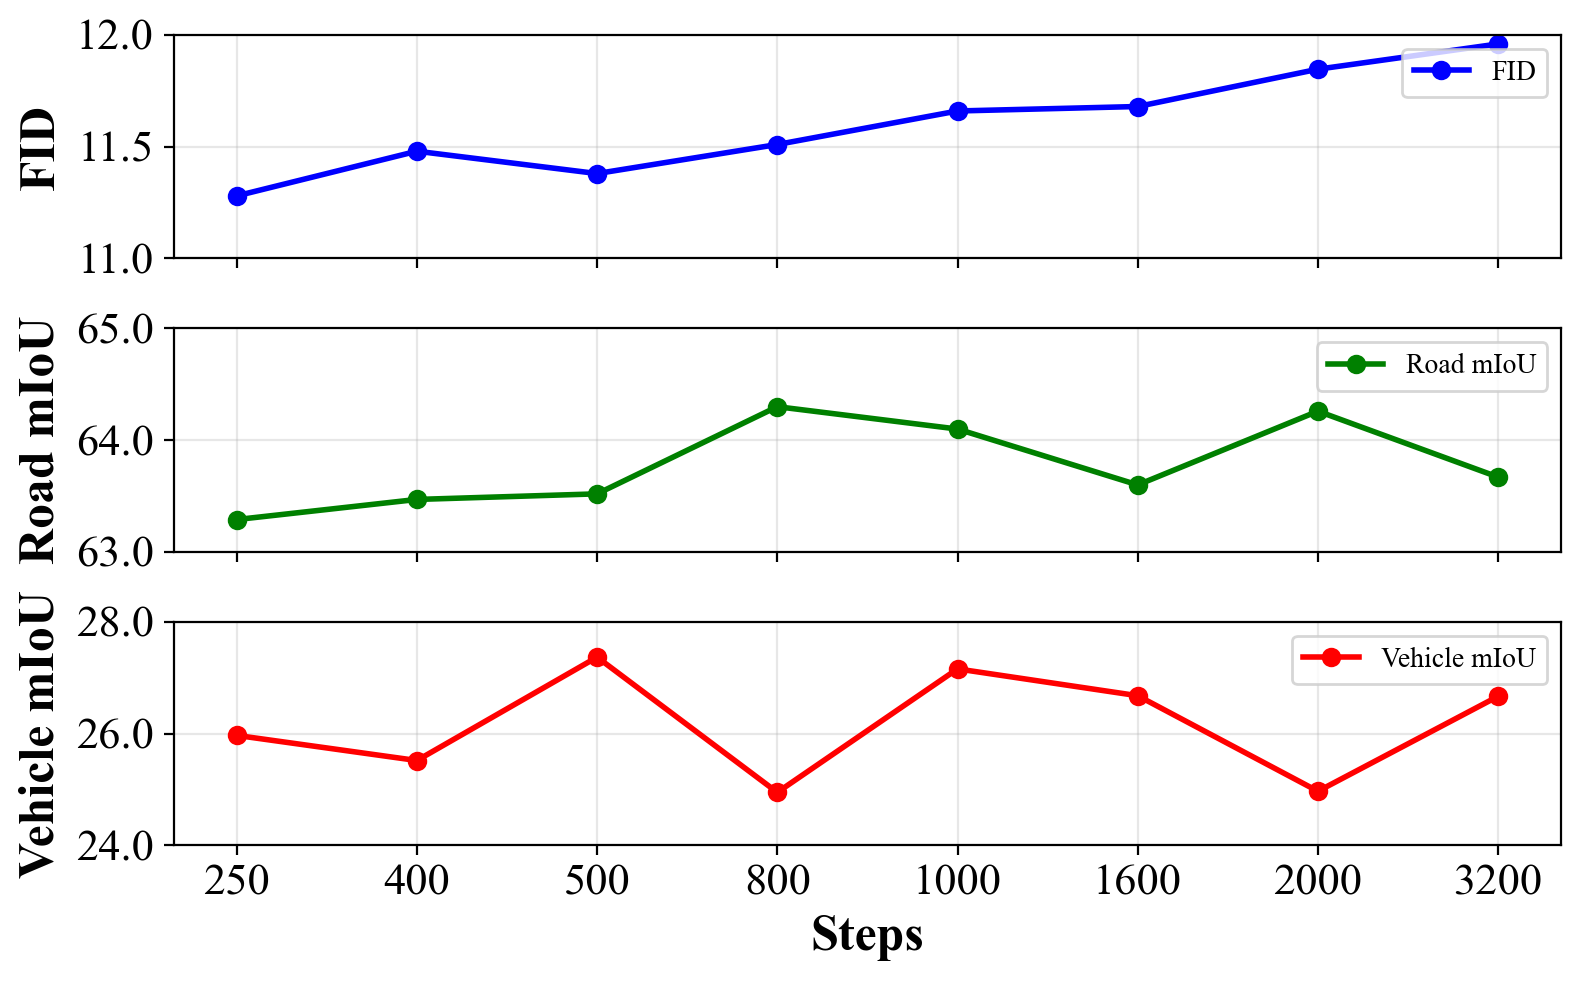
\includegraphics[width=0.45\textwidth]{ablation_steps_three_subplots.png}
	\caption{Impact of different iterative steps on the FID and geometry controllability of generated images.}
	\label{fig.5}
	\vspace{-8pt}
\end{figure}

\subsection{Visualisation Results}
\begin{figure}[h]
	\centering
	\includegraphics[width=0.45\textwidth]{add_split_compare_big.pdf}
	\caption{Examples of controllable road layout generation via HD map editing. Each row shows a case where the map is modified to introduce new road structures, with the generated image accurately reflecting these changes.}
	\label{fig.add_split_compare_big}
		\vspace{-5pt}
\end{figure}
\begin{figure}[h]
	\centering
	\includegraphics[width=0.48\textwidth]{vis-various-caption-new.pdf}
	\caption{Visualization of the impact of textual descriptions on scene reconstruction. Rows with the same index denote the same scene. Improvements brought by multi-view hierarchical  descriptions are highlighted with various colored circles or rectangles.}
	\label{fig.vis-various-caption}
		\vspace{-8pt}
\end{figure}
\begin{figure}[t]
	\centering
	\includegraphics[width=0.48\textwidth]{with-spatial-enhancement-loss.pdf}
	\caption{Qualitative comparison of scene generation with and without frequency-guided structure loss. Columns 1-2 show vehicle structure improvements, while columns 3-4 show road boundary enhancements. Red boxes highlight structural distortions without the proposed loss, whereas green boxes indicate successful mitigation with the loss.
	}
	\label{fig.with-spatial-enhancement-loss}
		\vspace{-5pt}
\end{figure}
\subsubsection{Controllable Road Layout Generation.}
Fig.~\ref{fig.add_split_compare_big} demonstrates controllable road layout generation through map editing across diverse scenarios.
Rows 1--2 show the transformation of static architectural regions into branch roads, showcasing the model's ability to synthesize plausible road structures in previously non-navigable areas.
Rows 3--4 present side road creation adjacent to parked vehicles, a challenging scenario where previous methods overfittingly link roadside parking with straight roads.
Rows 5--6 demonstrate intersection modifications, converting a T-junction into a four-way intersection by adding a road.
Rows 7--8 reveal the model's capacity to generate coherent road segments behind barriers such as fences and construction blocks, scenarios absent from existing datasets.
These results highlight the model's strong generalization capabilities and potential for creative scene synthesis. Extended examples are provided in the appendix, including cases of specific road deletion.
\subsubsection{Scene Reconstruction via Multi-view Hierarchical Descriptions.}
To evaluate the effect of textual details on scene generation, we compare images synthesized using default captions with those generated using our multi-view hierarchical descriptions. 
As shown in Fig.~\ref{fig.vis-various-caption}, our detailed descriptions lead to a more accurate reconstruction of key scene elements.
In Row 1, the red circle highlights a successfully recovered bus stop.
Row 2 shows a faithful reconstruction of a modern building and skybridge (yellow rectangle). 
In Row 3, a parking barrier gate (green circle) and blue multi-story residential building (green rectangle) are clearly restored. 
Moreover, when vehicle colors are explicitly mentioned, consistent results are generated, such as the red car in Row 2's back-right view and the white car in Row 3's back view.
These qualitative improvements demonstrate that our multi-view hierarchical descriptions significantly enhance the reconstruction of infrastructure, object attributes, and architectural details, which are elements often missed with default captions.
The superior visual quality observed in these examples corroborates our quantitative FID improvements.
\subsubsection{Visual Structure Improvement via Frequency-Guided Structure Loss. }
As demonstrated in Fig.~\ref{fig.with-spatial-enhancement-loss}, the incorporation of frequency-guided structure loss substantially improves the structural integrity and visual quality of generated scenes. 
Column 1 illustrates that the partially occluded white vehicle suffers from geometric distortions without this loss, while its shape is well-preserved when applying the frequency guidance. 
Column 2 reveals challenges in distant vehicle generation, where insufficient geometric cues lead to incomplete structures (red box), which are effectively restored through our proposed loss (green box).
Columns 3 and 4 examine structural improvements in road generation. The lack of high-frequency emphasis results in blurred and misaligned road boundaries (red box). 
Conversely, our frequency-guided structure loss recovers sharp contours and ensures better adherence to geometric layouts.
